\documentclass[UTF8,11pt,a4paper,oneside,fontset=none]{ctexart}

\usepackage[a4paper,top=1.75cm,bottom=1.75cm,left=1.85cm,right=1.85cm,headheight=15pt]{geometry}
\usepackage{fontspec}
\usepackage{amsmath,amssymb,mathtools,bm}
\usepackage{unicode-math}
\usepackage{booktabs,tabularx,array,multirow}
\usepackage[table]{xcolor}
\usepackage{graphicx,float}
\usepackage{siunitx}
\usepackage{enumitem}
\usepackage{fancyhdr}
\usepackage{caption}
\usepackage{hyperref}
\usepackage[most]{tcolorbox}
\usepackage{tikz}
\usetikzlibrary{arrows.meta,positioning,calc}

\setmainfont{Times New Roman}
\setsansfont{Arial}
\setmonofont{Consolas}
\setmathfont{Cambria Math}
\setCJKmainfont[BoldFont=SimHei,ItalicFont=KaiTi]{SimSun}
\setCJKsansfont[BoldFont={Microsoft YaHei Bold}]{Microsoft YaHei}
\setCJKmonofont{FangSong}

\definecolor{DeepBlue}{HTML}{17324D}
\definecolor{PandaTeal}{HTML}{0B7A75}
\definecolor{WarmGold}{HTML}{C58A19}
\definecolor{Coral}{HTML}{C95F4A}
\definecolor{SoftBlue}{HTML}{EEF5F8}
\definecolor{SoftTeal}{HTML}{ECF7F5}
\definecolor{SoftGold}{HTML}{FFF7E7}
\definecolor{SoftRed}{HTML}{FFF0F0}
\definecolor{MidGray}{HTML}{667085}
\definecolor{LineGray}{HTML}{D5DEE5}

\hypersetup{
  colorlinks=true,
  linkcolor=DeepBlue,
  urlcolor=PandaTeal,
  pdfauthor={范子恒},
  pdftitle={PandaX-4T 标定数据能量分辨率改善阶段性工作汇报：第一部分}
}

\ctexset{
  section={
    format=\Large\bfseries\color{DeepBlue},
    number=\arabic{section},
    beforeskip=0pt,
    afterskip=0.8em
  },
  subsection={format=\large\bfseries\color{PandaTeal}}
}

\pagestyle{fancy}
\fancyhf{}
\fancyhead[L]{\small\color{DeepBlue}PandaX-4T 能量分辨率改善}
\fancyhead[R]{\small\color{MidGray}阶段性汇报·第一部分}
\fancyfoot[C]{\small\color{MidGray}\thepage}
\renewcommand{\headrulewidth}{0.4pt}
\renewcommand{\footrulewidth}{0pt}

\captionsetup{font=small,labelfont=bf,labelsep=quad}
\graphicspath{{figures/}}
\setlength{\parindent}{2em}
\setlength{\parskip}{0.18em}
\setlist[itemize]{leftmargin=1.6em,itemsep=0.25em,topsep=0.25em,parsep=0pt}
\setlist[enumerate]{leftmargin=1.8em,itemsep=0.28em,topsep=0.25em,parsep=0pt}
\renewcommand{\arraystretch}{1.20}
\sisetup{
  group-separator={,},
  group-minimum-digits=4,
  range-phrase={--},
  range-units=single
}

\newcolumntype{Y}{>{\raggedright\arraybackslash}X}
\newcolumntype{C}[1]{>{\centering\arraybackslash}p{#1}}
\newcolumntype{R}[1]{>{\raggedleft\arraybackslash}p{#1}}

\newtcolorbox{keybox}[1][]{
  enhanced,breakable,
  colback=SoftBlue,colframe=DeepBlue,
  boxrule=0.7pt,arc=1.7mm,
  left=1.4mm,right=1.4mm,top=1.1mm,bottom=1.1mm,
  #1
}
\newtcolorbox{questionbox}[1][]{
  enhanced,breakable,
  colback=SoftGold,colframe=WarmGold,
  boxrule=0.8pt,arc=1.7mm,
  title={由数据提出的问题},fonttitle=\bfseries,
  left=1.4mm,right=1.4mm,top=1.0mm,bottom=1.0mm,
  #1
}
\newtcolorbox{scopebox}[1][]{
  enhanced,breakable,
  colback=SoftRed,colframe=Coral,
  boxrule=0.75pt,arc=1.7mm,
  title={结论边界},fonttitle=\bfseries,
  left=1.4mm,right=1.4mm,top=1.0mm,bottom=1.0mm,
  #1
}
\newtcolorbox{conclusionbox}[1][]{
  enhanced,breakable,
  colback=SoftTeal,colframe=PandaTeal,
  boxrule=0.85pt,arc=1.7mm,
  title={本页结论},fonttitle=\bfseries,
  left=1.4mm,right=1.4mm,top=1.0mm,bottom=1.0mm,
  #1
}

\newcommand{\Sone}{\mathrm{S1}}
\newcommand{\StwoB}{\mathrm{S2}_{\mathrm{B}}}
\newcommand{\Rsixtyeight}{R_{68}}
\newcommand{\Rninety}{R_{90}}
\newcommand{\OOF}{\mathrm{OOF}}

\begin{document}

% -----------------------------------------------------------------------------
% 封面
% -----------------------------------------------------------------------------
\thispagestyle{empty}
\vspace*{1.0cm}

\noindent{\color{PandaTeal}\rule{\textwidth}{3.5pt}}

\vspace{1.05cm}
{\sffamily\bfseries\fontsize{25pt}{32pt}\selectfont\color{DeepBlue}
PandaX-4T 标定数据\par
能量分辨率改善\par}

\vspace{0.35cm}
{\sffamily\bfseries\fontsize{18pt}{24pt}\selectfont\color{PandaTeal}
阶段性工作汇报\par}

\vspace{0.9cm}
\begin{tcolorbox}[
  colback=SoftBlue,colframe=DeepBlue,boxrule=0.9pt,arc=2mm,
  left=3mm,right=3mm,top=2.5mm,bottom=2.5mm
]
\centering
{\sffamily\bfseries\large 第一部分：从数据现象到问题定义}\par
\vspace{1mm}
本部分先回答“数据中看到了什么”和“下一步必须验证什么”，\par
不提前把诊断图解释成最终的分辨率改善结果。
\end{tcolorbox}

\vspace{0.75cm}
\begin{center}
\begin{tabular}{C{4.7cm} C{4.7cm} C{4.7cm}}
\begin{tcolorbox}[width=4.45cm,colback=white,colframe=LineGray,arc=1.5mm,halign=center]
{\sffamily\bfseries\fontsize{22pt}{24pt}\selectfont\color{DeepBlue}4500}\par
\small 事件
\end{tcolorbox}
&
\begin{tcolorbox}[width=4.45cm,colback=white,colframe=LineGray,arc=1.5mm,halign=center]
{\sffamily\bfseries\fontsize{22pt}{24pt}\selectfont\color{PandaTeal}188}\par
\small 输入变量
\end{tcolorbox}
&
\begin{tcolorbox}[width=4.45cm,colback=white,colframe=LineGray,arc=1.5mm,halign=center]
{\sffamily\bfseries\fontsize{22pt}{24pt}\selectfont\color{WarmGold}985}\par
\small 采集文件
\end{tcolorbox}
\end{tabular}
\end{center}

\vspace{0.45cm}
\begin{keybox}
\textbf{研究原则：}不直接采用已有重建结果或既有校正系数；从当前获得的输入变量重新建立校正、组合与验证流程。所有可学习参数都必须只由训练数据确定，再在未参与训练的数据上评价。
\end{keybox}

\vfill
\begin{tabularx}{\textwidth}{@{}Y R{5.2cm}@{}}
\textbf{汇报人：}范子恒 & \textbf{汇报日期：}2026 年 7 月 17 日\\
\textbf{数据：}run10972 & \textbf{项目：}Energy Resolution Improvement
\end{tabularx}

\vspace{0.35cm}
\noindent{\color{PandaTeal}\rule{\textwidth}{1.3pt}}
\clearpage

% -----------------------------------------------------------------------------
\section{数据样本与基本审计}

本项目当前拿到的是一个制表符分隔的标量文件，而不是未经处理的探测器波形。第一步不是立刻训练模型，而是确认样本规模、标识唯一性、关键变量的可用性以及结论能够覆盖的范围。

\vspace{0.35em}
\begin{minipage}[t]{0.54\textwidth}
\centering
\rowcolors{2}{SoftBlue}{white}
\begin{tabularx}{0.97\linewidth}{@{}Y R{3.35cm}@{}}
\toprule
\rowcolor{DeepBlue!11}\textbf{审计项目} & \textbf{结果}\\
\midrule
runNumber & 10972\\
事件数 & \num{4500}\\
变量数 & 188\\
不同 fileNumber 数 & 985\\
重复的 (run, file, event) & 0\\
完全缺失的变量 & 9\\
含无穷值的派生变量 & 18\\
关键基本变量有限值 & \num{4500}/\num{4500}\\
漂移时间范围 & \SIrange{10.1}{842.3}{\micro\second}\\
漂移时间中位数 & \SI{417.8}{\micro\second}\\
半径中位数 & \SI{359.1}{\milli\metre}\\
每个文件的事件数 & 1--14（中位数 4）\\
\bottomrule
\end{tabularx}
\end{minipage}\hfill
\begin{minipage}[t]{0.42\textwidth}
\begin{keybox}[title={本部分实际使用的变量},fonttitle=\bfseries]
\begin{itemize}
  \item 信号：\(qS1\_max\)、\(qS2B\_max\)；
  \item 深度信息：\(dt\)；
  \item 横向位置：\(xS2T\_max\)、\(yS2T\_max\)；
  \item 采集结构：\(runNumber\)、\(fileNumber\)、\(eventNumber\)。
\end{itemize}
这些基本变量在 4500 个事件中均为有限值。缺失值和无穷值主要出现在其他派生分支，后续不能无检查地全部送入模型。
\end{keybox}

\vspace{0.45em}
\begin{center}
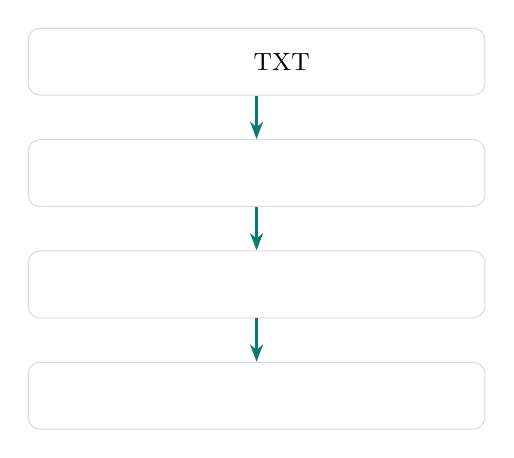
\begin{tikzpicture}[
  node distance=5.5mm,
  every node/.style={font=\small,align=center},
  box/.style={draw=LineGray,fill=white,rounded corners=1.5mm,minimum width=5.8cm,minimum height=8.5mm},
  arr/.style={-{Stealth[length=2.2mm]},thick,color=PandaTeal}
]
\node[box] (a) {读取上游标量 TXT};
\node[box,below=of a] (b) {检查单位、缺失值与无穷值};
\node[box,below=of b] (c) {检查事件标识和文件结构};
\node[box,below=of c] (d) {形成可复现的基本变量样本};
\draw[arr] (a)--(b);
\draw[arr] (b)--(c);
\draw[arr] (c)--(d);
\end{tikzpicture}
\end{center}
\end{minipage}

\vspace{0.65em}
\begin{scopebox}
文件名中的 \texttt{finalSS} 与 \texttt{Egt2MeV} 暗示样本很可能已经经过上游单散射及能量阈值等选择。因而本文把它称为“上游标量输入数据”，而不是“完全原始数据”。当前样本可以支持同一样本内的方法比较，但不能单独证明对所有探测器事件、所有能区都普遍有效。还需向数据提供方确认：\texttt{Egt2MeV} 的能量定义与效率、14 个 cut flag 的 0/1 含义，以及 fileNumber 是否严格对应采集顺序。
\end{scopebox}

\clearpage

% -----------------------------------------------------------------------------
\section{我们实际要改善什么？}

\subsection*{2.1 S1、S2 与联合能量}

粒子在液氙中沉积能量后，能量会分配到激发光子和电离电子两个通道。\(\Sone\) 是液相中的瞬发闪烁光；电子漂移到液面、被抽取到气相后产生电致发光，形成 \(\mathrm{S2}\)。本研究主要使用底部阵列记录的 \(\StwoB\)。

\begin{center}
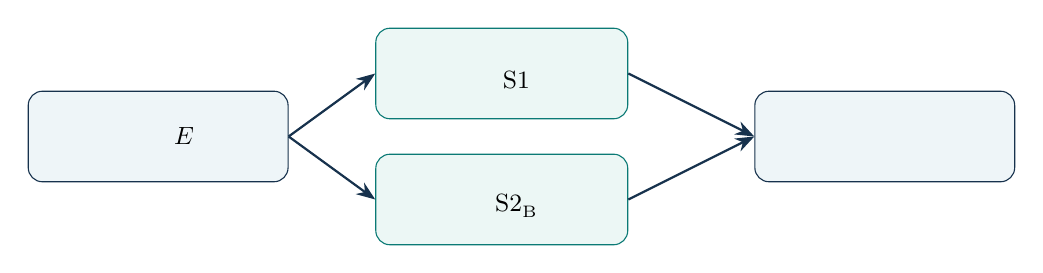
\begin{tikzpicture}[
  node distance=10mm and 11mm,
  every node/.style={font=\small,align=center},
  box/.style={draw=DeepBlue,fill=SoftBlue,rounded corners=1.8mm,minimum width=3.3cm,minimum height=1.15cm},
  sbox/.style={draw=PandaTeal,fill=SoftTeal,rounded corners=1.8mm,minimum width=3.2cm,minimum height=1.15cm},
  arr/.style={-{Stealth[length=2.4mm]},thick,color=DeepBlue}
]
\node[box] (e) {粒子沉积能量 \(E\)};
\node[sbox,right=of e,yshift=8mm] (s1) {激发光子\\观测为 \(\Sone\)};
\node[sbox,right=of e,yshift=-8mm] (s2) {电离电子漂移并抽取\\观测为 \(\StwoB\)};
\node[box,right=of s1,xshift=5mm,yshift=-8mm] (comb) {位置校正后联合\\重建能量};
\draw[arr] (e.east) -- (s1.west);
\draw[arr] (e.east) -- (s2.west);
\draw[arr] (s1.east) -- (comb.west);
\draw[arr] (s2.east) -- (comb.west);
\end{tikzpicture}
\end{center}

一种常见的物理表达是
\begin{equation}
  E
  =W\left(
    \frac{\Sone_{\mathrm{corr}}}{g_1}
    +\frac{\mathrm{S2}_{\mathrm{B,corr}}}{g_{2,\mathrm{B}}}
  \right),
\end{equation}
其中 \(W\) 是液氙中产生一个量子所需的平均能量，\(g_1\) 与 \(g_{2,\mathrm{B}}\) 是两个通道的探测增益。这里的公式说明研究方向，并不意味着本阶段已经假定这些参数已知。

\subsection*{2.2 “分辨率更好”如何量化？}

对重建能量 \(\widehat E\)，本文使用分位数定义的相对宽度：
\begin{align}
  \Rsixtyeight(\widehat E)
  &=\frac{Q_{0.84135}(\widehat E)-Q_{0.15865}(\widehat E)}
          {2Q_{0.5}(\widehat E)}\times 100\%,\\[0.35em]
  \Rninety(\widehat E)
  &=\frac{Q_{0.95}(\widehat E)-Q_{0.05}(\widehat E)}
          {2Q_{0.5}(\widehat E)}\times 100\%.
\end{align}

\begin{center}
\rowcolors{2}{SoftBlue}{white}
\begin{tabularx}{0.94\textwidth}{@{}C{2.1cm} Y Y@{}}
\toprule
\rowcolor{DeepBlue!11}\textbf{指标} & \textbf{直观含义} & \textbf{判断方式}\\
\midrule
\(Q_{0.5}\) & 能量分布的中位数，即分布中心 & 用作相对宽度的尺度\\
\(\Rsixtyeight\) & 覆盖中心约 68\% 事件的相对半宽 & 越小，中心峰越集中\\
\(\Rninety\) & 覆盖中心 90\% 事件的相对半宽 & 越小，宽尾和异常事件越少\\
\bottomrule
\end{tabularx}
\end{center}

\begin{questionbox}
什么才算“真正改善”？至少需要同时满足：\(\Rsixtyeight\) 与 \(\Rninety\) 下降；改善发生在未参与训练的事件上；不同位置和不同文件块中的结果保持一致。仅把训练数据压缩到一个常数附近不算有效重建。
\end{questionbox}

\begin{conclusionbox}
目标不是让某一张训练能谱看起来更尖，而是让独立测试数据中的中心宽度、尾部宽度和位置稳定性同时改善。
\end{conclusionbox}
\clearpage

% -----------------------------------------------------------------------------
\section{第一眼：四项基本数据观察}

\begin{figure}[H]
  \centering
  
\includegraphics[width=0.96\textwidth]{01_data_overview_cn.pdf}
  \caption{run10972 的四项基本观察。图中的“未在本项目中校正”表示尚未应用本项目重新学习的校正，不代表未经上游处理的波形原始量。}
\end{figure}

\vspace{-0.3em}
\rowcolors{2}{SoftBlue}{white}
\begin{tabularx}{\textwidth}{@{}C{0.8cm} Y Y@{}}
\toprule
\rowcolor{DeepBlue!11} & \textbf{图中直接看到什么} & \textbf{它提出了什么问题}\\
\midrule
(a) & \(\Sone\) 与 \(\StwoB\) 的点云总体向右下倾斜 & 两个通道能否互补并形成更窄的联合能量？\\
(b) & 漂移时间覆盖约 \SIrange{10.1}{842.3}{\micro\second}，但两端事件少 & 通道响应是否随深度变化？端点校正是否可靠？\\
(c) & 大部分事件集中在约 \SIrange{340}{390}{\milli\metre} & 位置趋势是否与源的空间分布混在一起？\\
(d) & 985 个文件中，每个文件通常只有 4 个事件 & 如何按文件分组验证，又不为单个文件单独拟合？\\
\bottomrule
\end{tabularx}

\vspace{0.45em}
\begin{conclusionbox}
四幅图共同说明：联合通道、位置依赖和采集文件结构都必须进入后续方法设计；但这些图本身还没有证明任何校正已经改善分辨率。
\end{conclusionbox}
\clearpage

% -----------------------------------------------------------------------------
\section{重点观察一：\texorpdfstring{\(\Sone\)--\(\StwoB\)}{S1--S2B} 反相关}

\begin{figure}[H]
  \centering
  
\includegraphics[width=0.94\textwidth]{02_s1_s2_anticorrelation_cn.pdf}
  \caption{每个点代表一个事件；横轴与纵轴分别是输入的 \(\Sone\) 和 \(\StwoB\)，颜色表示漂移时间。红线是按 \(\Sone\) 等频分箱后的中位数趋势。}
\end{figure}

\vspace{-0.2em}
\begin{minipage}[t]{0.48\textwidth}
\begin{keybox}[title={能够直接观察到},fonttitle=\bfseries]
\begin{itemize}
  \item 两个通道存在明确反相关：Pearson \(r=-0.575\)，Spearman \(\rho=-0.591\)；
  \item 分箱中位数趋势随 \(\Sone\) 增加而下降；
  \item 漂移时间颜色没有在点云内完全随机混合，说明深度与通道响应相关。
\end{itemize}
\end{keybox}
\end{minipage}\hfill
\begin{minipage}[t]{0.48\textwidth}
\begin{scopebox}[title={目前不能直接断言}]
\begin{itemize}
  \item 颜色差异不一定全部来自探测器响应；
  \item 源的位置分布、真实能量组成和上游选择也可能贡献趋势；
  \item 存在反相关不等于任意线性组合都会改善独立测试数据。
\end{itemize}
\end{scopebox}
\end{minipage}

\vspace{0.5em}
\begin{questionbox}
\textbf{问题 1：}在分别校正位置响应之后，\(\Sone\) 与 \(\StwoB\) 的联合量，能否在未参与训练的数据上同时得到更小的 \(\Rsixtyeight\) 和 \(\Rninety\)，并优于任一单通道？
\end{questionbox}

\begin{conclusionbox}
反相关为联合能量重建提供了数据依据；漂移时间结构则提示，在确定组合权重前必须先处理或同时建模位置响应。
\end{conclusionbox}
\clearpage

% -----------------------------------------------------------------------------
\section{重点观察二：空间覆盖并不均匀}

\begin{figure}[H]
  \centering
  
\includegraphics[width=0.94\textwidth]{03_spatial_coverage_cn.pdf}
  \caption{上图展示漂移时间；左下为输入横向位置的二维密度；右下为半径分布。虚线圆对应半径中位数，仅用于帮助观察空间结构。}
\end{figure}

\vspace{-0.25em}
\begin{itemize}
  \item \textbf{深度方向：}漂移时间覆盖较宽，中部统计量最高，两端较少；因此端点处的高自由度校正容易不稳定。
  \item \textbf{横向方向：}事件呈明显环状/边缘结构，径向中位数为 \SI{359.1}{\milli\metre}，四分位区间约为 \SIrange{345.7}{368.7}{\milli\metre}。其中 73.1\% 位于 \(340\le r<380\,\mathrm{mm}\)，而 \(r<200\,\mathrm{mm}\) 仅占 1.38\%。
  \item \textbf{直接后果：}样本没有均匀覆盖整个探测器；“位置相关响应”与“源本身的空间分布”可能相互混杂。
\end{itemize}

\begin{questionbox}
\textbf{问题 2：} \(\Sone\) 与 \(\StwoB\) 随漂移时间和半径的变化中，哪些可归因于探测器响应，哪些来自源分布或上游选择？

\textbf{问题 3：} 当前样本稀少或没有覆盖的空间区域，校正模型是否应当外推？怎样给出适用范围而不夸大结论？
\end{questionbox}

\begin{conclusionbox}
当前数据适合研究“本样本主要覆盖区域内”的相对校正；如果要声明全探测器适用，还需要更均匀的源样本或独立运行数据验证。
\end{conclusionbox}
\clearpage

% -----------------------------------------------------------------------------
\section{重点观察三：通道随位置的条件趋势}

为了减少单个散点的遮挡，将事件按漂移时间或半径分成 12 个等频箱；每个点画出该箱通道值的中位数，再除以全样本中位数。误差条表示分箱中位数的 68\% bootstrap 区间。

\begin{figure}[H]
  \centering
  
\includegraphics[width=0.98\textwidth]{04_conditional_trends_cn.pdf}
  \caption{输入通道的条件中位数趋势。它是诊断图，而不是已经确定的探测器响应函数或最终校正曲线。}
\end{figure}

\begin{minipage}[t]{0.48\textwidth}
\begin{keybox}[title={图中现象},fonttitle=\bfseries]
随漂移时间增加，\(\Sone\) 的条件中位数总体上升，而 \(\StwoB\) 总体下降；描述性的 Pearson 系数分别为 \(r(t_{\mathrm d},\Sone)=+0.665\) 与 \(r(t_{\mathrm d},\StwoB)=-0.686\)。半径接近样本外缘时也出现明显且相反的变化，趋势幅度明显大于分箱中位数的统计误差。
\end{keybox}
\end{minipage}\hfill
\begin{minipage}[t]{0.48\textwidth}
\begin{scopebox}[title={解释限制}]
这里只做了“在某位置条件下观察到什么”的描述。由于位置、源分布、真实能量与上游选择可能相关，不能把整条曲线直接当作纯探测器响应，更不能用任意高阶函数把趋势全部抹平。
\end{scopebox}
\end{minipage}

\vspace{0.55em}
\begin{questionbox}
\textbf{问题 4：}能否使用低自由度、可解释的响应函数校正深度和半径趋势，并且只在训练文件上确定参数、在测试文件上冻结应用，从而避免把源分布和统计涨落学进校正？
\end{questionbox}

\begin{conclusionbox}
位置趋势确实需要处理，但校正的目标必须由独立测试数据上的分辨率与平坦性共同约束，而不是让训练图中的曲线看起来完全水平。
\end{conclusionbox}
\clearpage

% -----------------------------------------------------------------------------
\section{验证原则与本部分形成的问题}

\begin{figure}[H]
  \centering
  
\includegraphics[width=0.90\textwidth]{05_file_structure_cn.pdf}
  \caption{单个采集文件的事件很少，因此不适合为每个文件独立拟合；但 fileNumber 仍应作为训练/测试分组的基本单位。右图颜色仅示意五个连续文件块。}
\end{figure}

\vspace{-0.25em}
\subsection*{7.1 为什么不能简单随机拆分事件？}

同一采集文件中的事件可能共享相同的时间状态或运行条件。如果把同一文件中的事件随机分到训练集和测试集两边，模型可能通过文件特征间接“看见”测试条件，造成信息泄漏。因此采用以下验证链条：

\begin{center}
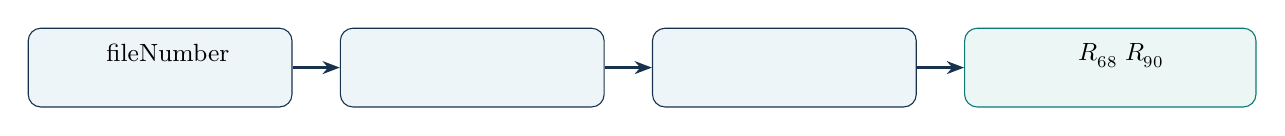
\begin{tikzpicture}[
  node distance=6mm,
  every node/.style={font=\small,align=center},
  box/.style={draw=DeepBlue,fill=SoftBlue,rounded corners=1.6mm,minimum width=3.35cm,minimum height=1.0cm},
  last/.style={draw=PandaTeal,fill=SoftTeal,rounded corners=1.6mm,minimum width=3.7cm,minimum height=1.0cm},
  arr/.style={-{Stealth[length=2.2mm]},thick,color=DeepBlue}
]
\node[box] (a) {按 fileNumber\\分组};
\node[box,right=of a] (b) {训练文件\\学习校正与组合参数};
\node[box,right=of b] (c) {冻结参数并应用到\\未参与训练的文件};
\node[last,right=of c] (d) {比较 \(\Rsixtyeight\)、\(\Rninety\)\\及位置稳定性};
\draw[arr] (a)--(b);
\draw[arr] (b)--(c);
\draw[arr] (c)--(d);
\end{tikzpicture}
\end{center}

\subsection*{7.2 第一部分最终形成的五个可检验问题}

\begin{enumerate}[label=\textbf{Q\arabic*.}]
  \item 校正后的 \(\Sone\) 与 \(\StwoB\) 联合重建，能否优于任一单通道？
  \item 漂移时间和径向位置效应应如何分离、校正并限制自由度？
  \item 空间覆盖不均是否限制模型的适用范围与外推能力？
  \item 改善是否同时出现在中心宽度 \(\Rsixtyeight\) 和尾部宽度 \(\Rninety\) 上？
  \item 改善是否出现在未参与训练的文件，以及更严格的连续文件块测试中？
\end{enumerate}

\begin{keybox}[title={第一部分已经完成了什么？},fonttitle=\bfseries]
\begin{itemize}
  \item 从实际 TXT 数据完成了样本、缺失值、事件标识和文件结构审计；
  \item 生成并解释了 5 组中文诊断图，确认反相关、非均匀空间覆盖和明显条件趋势；
  \item 明确了不能从当前图像直接得出的结论，并把后续工作转化为五个可检验问题；
  \item 确定后续所有模型都必须采用按采集文件分组的样本外验证。
\end{itemize}
\end{keybox}

\begin{conclusionbox}
\textbf{汇报收束句：}目前我们还没有把某个数字当作最终答案；但已经从数据事实出发，明确了为什么需要联合重建、为什么需要位置校正，以及用什么规则判断后续改善不是过拟合。下一部分将据此汇报候选方法、样本外结果和仍然存在的限制。
\end{conclusionbox}

\end{document}
